\documentclass{article}
\usepackage{graphicx} % Required for inserting images
\usepackage[top=0.9in, bottom=1in, left=1.5in, right=1.5in]{geometry}
\usepackage[utf8]{inputenc}
\usepackage[icelandic]{babel}
\usepackage[T1]{fontenc}
\usepackage[sc]{mathpazo}
\usepackage[parfill]{parskip}
\renewcommand{\baselinestretch}{1.2}
% Tables and lists
\usepackage{booktabs,tabularx}
\usepackage{multirow}
\usepackage{enumerate}
\usepackage{adjustbox}
\usepackage{multicol}
\usepackage{xcolor}
\usepackage{algpseudocode}
\usepackage{tikz}
\usepackage{nicefrac}
\usepackage{changepage}
\usetikzlibrary{arrows, positioning, calc, graphs}

% Math
\usepackage{amsmath, amsfonts, amssymb, amsthm}
% Graphics

\usepackage{graphicx}
\usepackage{tikz}
% Code environment
\usepackage{minted}
%\usepackage{bm}
%\usepackage{siunitx}
%\usepackage{animate}
%\usepackage{hyperref}
%\usepackage{movie15}
%\usepackage{multicol}
%\usepackage{changepage}
\title{Formal Languages and Computability 2}
\author{Ragnar Björn Ingvarsson, rbi3}
\tikzset{->, >=stealth', shorten >=1pt, node distance=2cm,thick, main node/.style={circle,draw,minimum size=3em}}


\begin{document}
\renewcommand\thepage{}
	
	\maketitle

	\newpage
	\setcounter{page}{1}
	\renewcommand\thepage{\arabic{page}}
	\section{Which of the statements are true for every regular language 
	A?}

	\begin{itemize}
		\item[a)]\textit{A = A*} 

			For this case we see that the empty string, $\epsilon$ is not 
			neccessarily in $A$, however it is guaranteed to be a 
			possibility within $A^*$. 

			Therefore these are not always equal.
		\item[b)]\textit{A* = A $\circ$ A*}

			We see here that it is possible to say that $A=\{0,1\}$ for 
			example, and then the left side can become just the empty 
			string, but the right side must contain a $0$ or a $1$ before 
			it can give the empty string, rendering it useless.

			Therefore these are not always equal.
		\item[c)]\textit{A* $\circ$ A = A $\circ$ A*}

			Here we notice that the empty string, $\epsilon$, has no effect 
			since both sides contain at least one character. Because of 
			this, there is no possible string that one side can construct 
			that the other cannot.

			So this statement is \textit{true}.
	\end{itemize}

	\section{Let $\Sigma=\{0,1\}$ and let $A$ denote a language of 
		strings that consist soley of any number of zeroes, or at most 
	two ones, including the empty string.}

	\begin{itemize}
		\item[a)] Draw a state diagram of an NFA that recognizes $A$.

			\vspace{2.5em}
			\begin{center}
			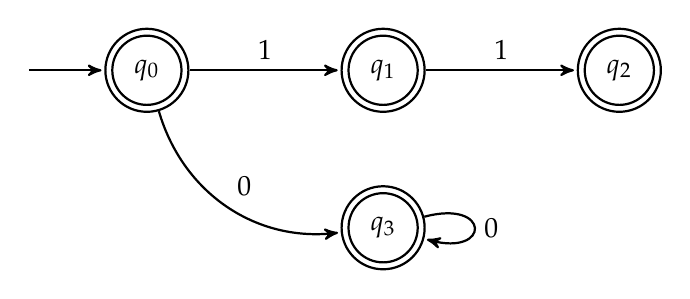
\begin{tikzpicture}[thick, auto]
				\node[main node] (q0) {$q_0$};
				\node[main node,minimum size=2.5em] (q0fin) {};
				\node[main node] at (3,0) (q1) {$q_1$};
				\node[main node,minimum size=2.5em] at (3,0) (q1fin) {};
				\node[main node] at (6,0) (q2) {$q_2$};
				\node[main node,minimum size=2.5em] at (6,0) (q2fin) {};
				\node[main node] at (3,-2) (q3) {$q_3$};
				\node[main node,minimum size=2.5em] at (3,-2) (q3fin) {};

				\path (-1.5,0) edge node {} (q0);
				\path (q0) edge node {$1$} (q1);
				\path (q1) edge node {$1$} (q2);
				\path (q0) edge[bend right=40] node {$0$} (q3);
				\path (q3) edge[loop right=20] node {$0$} (q3);
			\end{tikzpicture}
			\end{center}

			\newpage
		\item[b)] How many states do you need with a DFA to do the same 
			task?

			You simply need one extra state, a sort of \textit{purgatory 
			state}, where to there exists a path from all states but $q_0$ 
			on the 'incorrect' input.

			So we can say that in a) we have two 
			paths, the $0$ path and the $1$ path. We'll then include paths 
			to the purgatory state on $1$'s on the $0$ path and 
			vice versa. Finally, we'll have the purgatory state 
			loop back on itself on both $0$ and $1$ while not being an 
			exit state:

			\vspace{2em}
			\begin{center}
			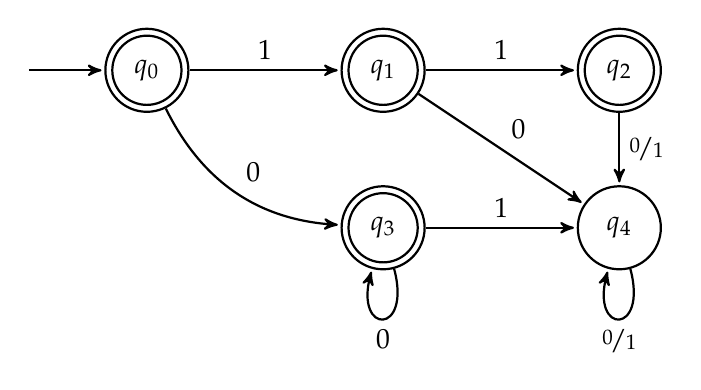
\begin{tikzpicture}[thick, auto]
				\node[main node] (q0) {$q_0$};
				\node[main node,minimum size=2.5em] (q0fin) {};
				\node[main node] at (3,0) (q1) {$q_1$};
				\node[main node,minimum size=2.5em] at (3,0) (q1fin) {};
				\node[main node] at (6,0) (q2) {$q_2$};
				\node[main node,minimum size=2.5em] at (6,0) (q2fin) {};
				\node[main node] at (3,-2) (q3) {$q_3$};
				\node[main node,minimum size=2.5em] at (3,-2) (q3fin) {};
				\node[main node] at (6,-2) (q4) {$q_4$};

				\path (-1.5,0) edge node {} (q0);
				\path (q0) edge node {$1$} (q1);
				\path (q1) edge node {$1$} (q2);
				\path (q0) edge[bend right=30] node {$0$} (q3);
				\path (q3) edge[loop below=20] node {$0$} (q3);
				\path (q1) edge node {$0$} (q4);
				\path (q2) edge node {$\nicefrac{0}{1}$} (q4);
				\path (q3) edge node {$1$} (q4);
				\path (q4) edge[loop below=20] node 
				{$\nicefrac{0}{1}$} (q4);
			\end{tikzpicture}
			\end{center}
	\end{itemize}

	\section{Consider the ternary number system.}

	\begin{itemize}
		\item[a)] Draw a state diagram for a DFA that accepts ternary 
			strings that are \textit{not} divisible by three.

		\vspace{2em}
		\begin{center}
		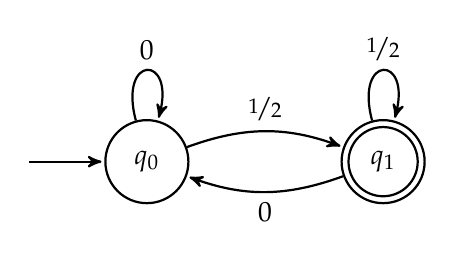
\begin{tikzpicture}[thick, auto]
			\node[main node] (q0) {$q_0$};
			\node[main node] at (3,0) (q1) {$q_1$};
			\node[main node,minimum size=2.5em] at (3,0) (q1fin) {};

			\path (-1.5,0) edge node {} (q0);
			\path (q0) edge[loop above=20] node {0} (q0);
			\path (q0) edge[bend left=20] node {\nicefrac{1}{2}} (q1);
			\path (q1) edge[bend left=20] node {0} (q0);
			\path (q1) edge[loop above=20] node {\nicefrac{1}{2}} (q1);
		\end{tikzpicture}
		\end{center}
		\vspace{2em}

		\newpage
		\item[b)] Draw a state diagram for a DFA that accepts ternary 
			strings that are \textit{not} divisible by nine.

			\vspace{1.5em}
			\begin{center}
			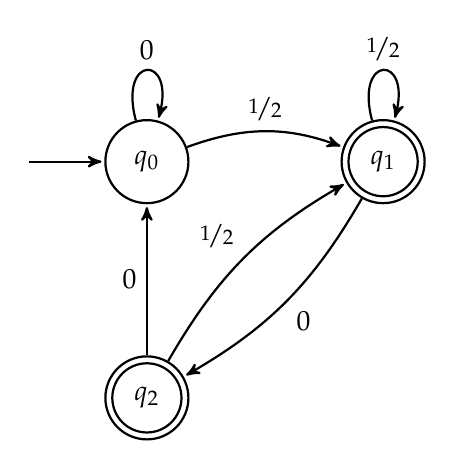
\begin{tikzpicture}[thick, auto]
				\node[main node] (q0) {$q_0$};
				\node[main node] at (0,-3) (q2) {$q_2$};
				\node[main node,minimum size=2.5em] at (0,-3) (q2fin) {};
				\node[main node] at (3,0) (q1) {$q_1$};
				\node[main node,minimum size=2.5em] at (3,0) (q1fin) {};

				\path (-1.5,0) edge node {} (q0);
				\path (q0) edge[loop above=20] node {0} (q0);
				\path (q0) edge[bend left=20] node {\nicefrac{1}{2}} (q1);
				\path (q1) edge[loop above=20] node {\nicefrac{1}{2}} (q1);
				\path (q1) edge[bend left=15] node {0} (q2);
				\path (q2) edge[bend left=15] node {\nicefrac{1}{2}} (q1);
				\path (q2) edge node {0} (q0);
			\end{tikzpicture}
			\end{center}
			\vspace{2em}
	\end{itemize}

	\section{Design a finite state automata that accepts binary numbers 
		corresponing to perfect squares that can give false positives, 
	but not false negatives.}

	\begin{itemize}
		\item[a)] Show that $n^2$ mod $3 \neq 2$ for all $n = 0,1,2,...$

			We prove by induction.

			Base case $k=0$ shows that $0^2$ mod $3 = 0$ mod $3 = 0 \neq 2$

			So we continue. \\ Lets assume that the statement is true for 
			some $k \in \mathbb{N}$ so that $k^2$ mod $3 \neq 2$. \\ 
			Then: $(k+1)^2$ mod $3 \\ = k^2 + 2k + 1$ mod $3 \\ = ((k^2$ mod 
			$3) + (2k + 1$ mod $3))$ mod $3$
			$\\ = ((k^2$ mod $3) + (2k$ mod $3) + (1$ mod $3))$ mod $3$
			$\\ = ((k^2$ mod $3) + 1 + (2k$ mod $3))$ mod $3$

			We see here that since $k^2$ mod $3 \neq 2$, then $k^2$ mod $3$ 
			is either $0$ or $1$.

			\begin{itemize}
				\item[]$k^2$ mod $3 = 0$: Here we get 
					\[(2k\text{ mod }3 + 1)\text{ mod }3\]
					And since $k^2$ mod $3 = 0$, we notice that the prime 
					factors of $k^2$ must include $3^2$, one for each $k$.
					Therefore $k$ mod $3 = 0$ must also be true, 
					and then $2k$ mod $3 = 0$.

					So $(2k$ mod $3 + 1)$ mod $3 = 1$ mod $3 = 1 \neq 2$
				\item[]$k^2$ mod $3 = 1$: Here we get
					\[(2k\text{ mod }3 + 2)\text{ mod }3\]
					And since $k^2$ mod $3 = 1$ we see that the prime 
					factors of $k^2$ must \textit{not} include $3$. 
					Therefore, $k$ mod $3 \neq 0$ so that $2k$ mod 
					$3 \neq 0$ so 

					\[2k \text{ mod } 3 = 1 \text{ or } 2k 
					\text{ mod } 3 = 2\]

					So we get 
					\[(2k \text{ mod } 3 + 2) \text{ mod } 3\]
					\[= (1 + 2) \text{ mod } 3\]
					\[= 0\]
					Or 
					\[(2k \text{ mod } 3 + 2) \text{ mod } 3\]
					\[= (2 + 2) \text{ mod } 3\]
					\[= 1\]

					Both of which are not $2$. So $(k+1)^2 \text{ mod } 3 
					\neq 2$. 

					$\hfill\blacksquare$

			\end{itemize}
		\item[b)] By using the above result, design a DFA/NFA that rejects 
			$33\%$ of all possible numbers without any false negatives. 
			Submit the state diagram of your automata.

			We notice that the DFA for binary numbers that are divisible 
			by $3$ is as follows:

			\begin{center}
			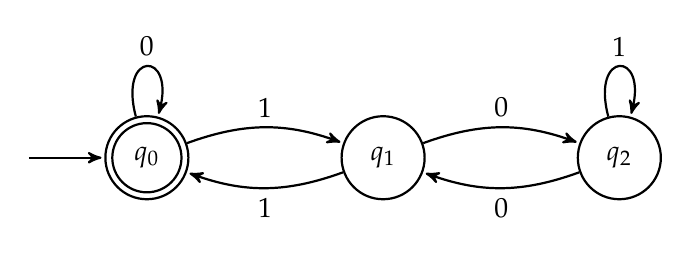
\begin{tikzpicture}[thick,auto]
				\node[main node] (q0) {$q_0$};
				\node[main node,minimum size=2.5em] (q0fin) {};
				\node[main node] at (3,0) (q1) {$q_1$};
				\node[main node] at (6,0) (q2) {$q_2$};

				\path (-1.5,0) edge node {} (q0);
				\path (q0) edge[loop above=20] node {$0$} (q0);
				\path (q0) edge[bend left=20] node {$1$} (q1);
				\path (q1) edge[bend left=20] node {$1$} (q0);
				\path (q1) edge[bend left=20] node {$0$} (q2);
				\path (q2) edge[bend left=20] node {$0$} (q1);
				\path (q2) edge[loop above=20] node {$1$} (q2);
			\end{tikzpicture}
			\end{center}

			And to satisfy the requirement we only need to accept numbers 
			that, when divided by $3$, do not give a remainder of $2$.

			Therefore, as the automata works with each state signifying 
			what the current remainder of the number is, we just need 
			to make $q_1$ an exit state along with $q_0$ and that only 
			leaves numbers giving a remainder of $2$ behind.

			\begin{center}
			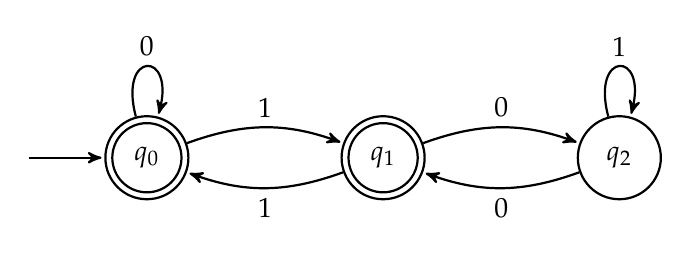
\begin{tikzpicture}[thick,auto]
				\node[main node] (q0) {$q_0$};
				\node[main node,minimum size=2.5em] (q0fin) {};
				\node[main node] at (3,0) (q1) {$q_1$};
				\node[main node,minimum size=2.5em] at (3,0) (q1fin) {};
				\node[main node] at (6,0) (q2) {$q_2$};

				\path (-1.5,0) edge node {} (q0);
				\path (q0) edge[loop above=20] node {$0$} (q0);
				\path (q0) edge[bend left=20] node {$1$} (q1);
				\path (q1) edge[bend left=20] node {$1$} (q0);
				\path (q1) edge[bend left=20] node {$0$} (q2);
				\path (q2) edge[bend left=20] node {$0$} (q1);
				\path (q2) edge[loop above=20] node {$1$} (q2);
			\end{tikzpicture}
			\end{center}

	\end{itemize}

\end{document}
